\documentclass[12pt, letterpaper]{article}
\usepackage{graphicx} %Latex package to import graphics (i.e. images)
\usepackage{forest} %Latex package to draw tree diagram
\usepackage{subfigure} %Latex package to provide support for small figures
\usepackage{amsmath}
\graphicspath{{etc}}
\title{Why is $ \frac{\partial J(W)}{\partial W_{i,j}^{(out)}} = (A^{(h)})^{T} \delta^{(out)}$ ?}
\author{Kassi Bertrand}
\date{January $19^{th}$, 2023}

\begin{document}
\maketitle

\section{Introduction}
In this \LaTeX{} document, I want to show my step-by-step process
to derive the partial derivative of the loss function with respect
to of all the weights in $W^{(out)}$.

\vspace{5mm} %5mm vertical space

I'll start simple with a 2-2-2 MLP, which is a Multi-Layer Perceptron
with 2 inputs, 2 hidden units, and 2 outputs, and then generalize
what we learn to a general $m-d-t$ MLP.

\vspace{5mm} %5mm vertical space

In both cases, I will use the following loss/error function:
\[J(w) = -\sum\nolimits_{i = 1}^{n}\sum\nolimits_{j=1}^{t} y_j^{[i]} ln(a_j^{[i]}) + (1 - y_j^{[i]})ln(1 - a_j^{[i]})\]

Where the superscript $[i]$ is an index for training examples,
and $j$ is the number of output units.

\vspace{5mm} %5mm vertical space

Ready? Let's go!

\pagebreak
\section{With a 2-2-2 MLP}

For this example, we will consider the following Neural network:

%2-2-2 MLP picture
\begin{center}
    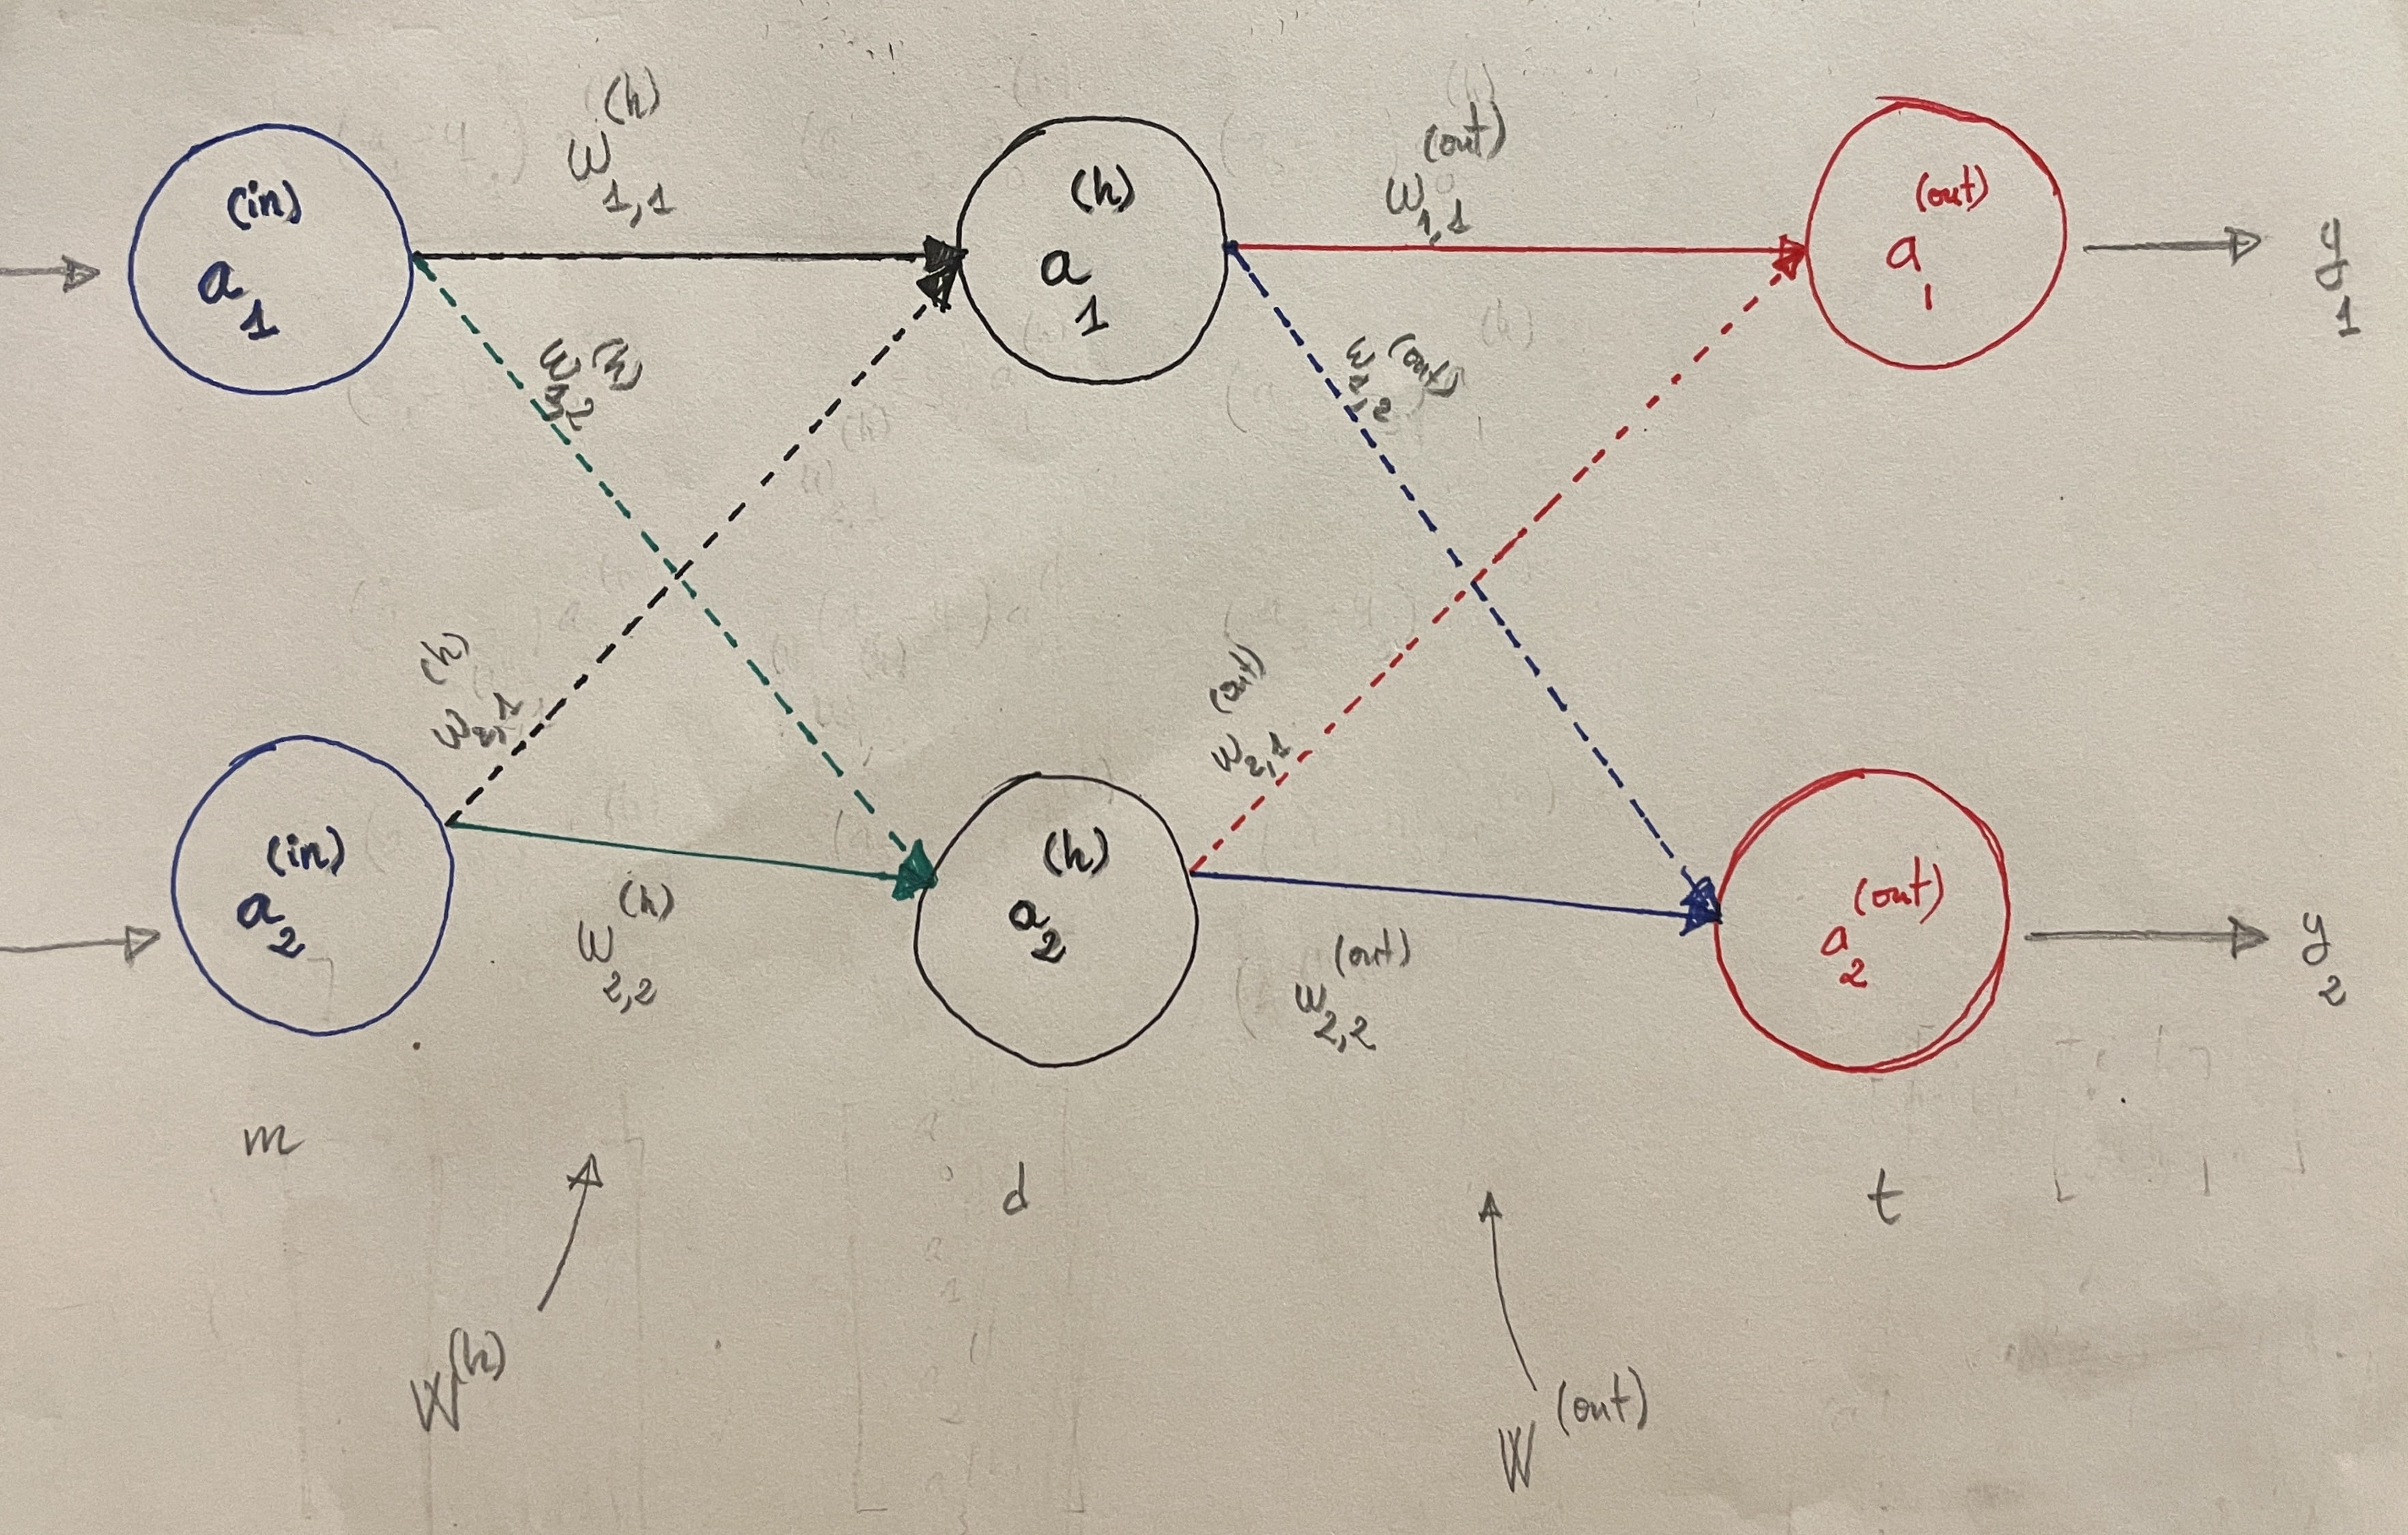
\includegraphics[width = 16cm, height = 9cm]{2-2-2-mlp.jpg}
\end{center}

\vspace{5mm} %5mm vertical space

We'll ignore biase units in the input and hidden layers, and 
consider only ONE training example for simplicity purposes.

\vspace{5mm} %5mm vertical space

Since one training example is considered and the network has
two activation units in its output layer, then  $n = 1$ and 
$t = 2$. So, the loss function becomes like this:

\[J(w) = -\sum\nolimits_{i = 1}^{1}\sum\nolimits_{j=1}^{2} y_j^{[i]} ln(a_j^{[i]}) + (1 - y_j^{[i]})ln(1 - a_j^{[i]})\]

\vspace{5mm} %5mm vertical space

The journey of a SINGLE training example from the input layer to
the output layer of our network goes like this:

\vspace{5mm} %5mm vertical space

\pagebreak
\[[a_1^{(in)}, a_2^{(in)}]\]
\[\downarrow\]
\[W^{(h)}\]
\[\downarrow\]                  
\[[z_1^{(h)}, z_2^{(h)}]\]
\[\downarrow\]
\[\phi(\bullet)\]
\[\downarrow\]
\[[a_1^{(h)}, a_2^{(h)}]\]
\[\downarrow\]
\[W^{(out)}\]
\[\downarrow\]                  
\[[z_1^{(out)}, z_2^{(out)}]\]
\[\downarrow\]
\[\phi(\bullet)\]
\[\downarrow\]
\[[a_1^{(out)}, a_2^{(out)}]\]
\[\downarrow\]
\[[y_1, y_2]\]
\pagebreak

Now, let's compute the partial derivative of $J(W)$ w.r.t to
each  weights in the $W^{(out)}$ matrix. To help myself, 
I drew the following tree diagram to see how the variables 
in $J(W)$ relate to the weights in $W^{(out)}$:

\vspace{5mm} %5mm vertical space

\begin{figure}[h!]
    \centering
    \begin{forest}
        for tree={
            l sep=30pt,
            parent anchor=south,
            align=center
        }
            [$J(W)$
                [$y_1^{[i]}$]
                [$a_1^{[i]}$
                    [$z_1^{[i]}$
                        [$w_{1,1}^{(out)}$]
                        [$w_{2,1}^{(out)}$]
                    ]
                ]
                [$y_2^{[i]}$]
                [$a_2^{[i]}$
                    [$z_2^{[i]}$
                        [$w_{1,2}^{(out)}$]
                        [$w_{2,2}^{(out)}$]
                    ]
                ]
            ]
    \end{forest}
\end{figure}

Our MLP has two outputs, and if you look at $J(W)$ 
closely, you'll see that it's a \textbf{sum}. So, we compute 
the cost for \underline{each} output, then add the results together. 
And that's how we get the cost for the current training
example. With that in mind, we can now compute the partial
derivatives:

\vspace{5mm} %5mm vertical space

\[
    \frac{\partial J(W)}{\partial w_{1,1}^{(out)}} = 
    \frac{\partial J(W)}{\partial a_{1}^{(out)}} \times
    \frac{\partial a_{1}^{(out)}}{\partial z_{1}^{(out)}} \times
    \frac{\partial z_{1}^{(out)}}{\partial w_{1,1}^{(out)}}
\]

\[
    \frac{\partial J(W)}{\partial w_{2,1}^{(out)}} = 
    \frac{\partial J(W)}{\partial a_{1}^{(out)}} \times
    \frac{\partial a_{1}^{(out)}}{\partial z_{1}^{(out)}} \times
    \frac{\partial z_{1}^{(out)}}{\partial w_{2,1}^{(out)}}
\]

\[
    \frac{\partial J(W)}{\partial w_{1,2}^{(out)}} = 
    \frac{\partial J(W)}{\partial a_{2}^{(out)}} \times
    \frac{\partial a_{2}^{(out)}}{\partial z_{2}^{(out)}} \times
    \frac{\partial z_{2}^{(out)}}{\partial w_{1,2}^{(out)}}
\]

\[
    \frac{\partial J(W)}{\partial w_{2,2}^{(out)}} = 
    \frac{\partial J(W)}{\partial a_{2}^{(out)}} \times
    \frac{\partial a_{2}^{(out)}}{\partial z_{2}^{(out)}} \times
    \frac{\partial z_{2}^{(out)}}{\partial w_{2,2}^{(out)}}
\]

\vspace{5mm} %5mm vertical space

Notice, the following expressions are common in the first two and
last two equations. Let's evaluate them:

\[
    \frac{\partial J(W)}{\partial a_{1}^{(out)}} \times
    \frac{\partial a_{1}^{(out)}}{\partial z_{1}^{(out)}} = 
    (a_{1}^{(out)} - y_1) = \delta_1^{(out)}
\]

\[
    \frac{\partial J(W)}{\partial a_{2}^{(out)}} \times
    \frac{\partial a_{2}^{(out)}}{\partial z_{2}^{(out)}} = 
    (a_{2}^{(out)} - y_2) = \delta_2^{(out)}
\]

\vspace{5mm} %5mm vertical space

$(a_{1}^{(out)} - y_1)$ and $(a_{2}^{(out)} - y_2)$ are the 
``\textbf{error}" terms in the output layer. Since our MLP
has two outputs, we have two ``error" terms as well. We use 
``$\delta$" to denote that ``error". $\delta_1^{(out)}$ for 
instance, is the error in the first activation unit in the 
output layer.

\vspace{5mm} %5mm vertical space

With this new knowledge, we can re-write the partial derivatives:

\[
    \frac{\partial J(W)}{\partial w_{1,1}^{(out)}} =
    \delta_1^{(out)} a_1^{(h)}
\]

\[
    \frac{\partial J(W)}{\partial w_{2,1}^{(out)}} =
    \delta_1^{(out)} a_2^{(h)}
\]

\[
    \frac{\partial J(W)}{\partial w_{1,2}^{(out)}} =
    \delta_2^{(out)} a_1^{(h)}
\]

\[
    \frac{\partial J(W)}{\partial w_{2,2}^{(out)}} =
    \delta_2^{(out)} a_2^{(h)}
\]

From the above, I can now introduce the $\delta^{(out)}$ matrix.
It is our ``error'' matrix, and is of the shape $n \times t$ 
where $n$ is the number of training examples and $t$ the number 
of activation units in the output layer. Since we are dealing with
\underline{ONE} example and our MLP has \underline{2} outputs, so 
the $\delta^{(out)}$ matrix is of the shape $(1 \times 2)$, and 
looks like this:

\[
    \delta^{(out)} = [\delta_1^{(out)}, \delta_2^{(out)}] =
    [(a_{1}^{(out)} - y_1), (a_{2}^{(out)} - y_2)]
\]

\vspace{5mm} %5mm vertical space

Also, remember the $A^{(h)}$ matrix, obtained after training
examples are forward propagated from the input to the hidden layer.
It is a $(n \times d)$ matrix; where $n$ is the number of training
examples and $d$ the number of activation units in the hidden layer.
Since we have \underline{ONE} training example and \underline{2}
units in the hidden layer, our $A^{(h)}$ matrix is of the shape
$(1 \times 2)$, and looks like this:

\[
    A^{(h)} = [a_1^{[1]}, a_2^{[1]}]
\]

We computed the partial derivatives with respect to the weights in
$W^{(out)}$ above. But we can implement the same operations in 
vectorized form? Yes, of course! Look at this:

\[
    (A^{(h)})^{T} \delta^{(out)}
    =
    \begin{bmatrix}
        a_1^{[1]} \\
        a_2^{[1]}
    \end{bmatrix}
    \times
    \begin{bmatrix}
        \delta_1^{(out)} & \delta_2^{(out)}
    \end{bmatrix}
    = 
    \begin{bmatrix}
        a_1^{(h)} \delta_1^{(out)} & a_2^{(h)} \delta_1^{(out)} \\
        a_1^{(h)} \delta_2^{(out)} & a_2^{(h)} \delta_2^{(out)}
    \end{bmatrix}
\]

See? By transposing the $A^{(h)}$ and multiplying it with
$\delta^{(out)}$, we obtain a new matrix containing the partial
derivatives of $J(W)$ w.r.t to each weights in $W^{(out)}$.

\vspace{5mm} %5mm vertical space

We can see that for our 2-2-2 MLP, $\frac{\partial J(W)}
{\partial W_{i,j}^{(out)}} = (A^{(h)})^{T} \delta^{(out)}$.
Can we show this relationship holds for a general MLP?

\pagebreak
\section{With a general $m-d-t$ MLP}

Let's consider a general MLP like the following:

%General MLP picture
\begin{center}
    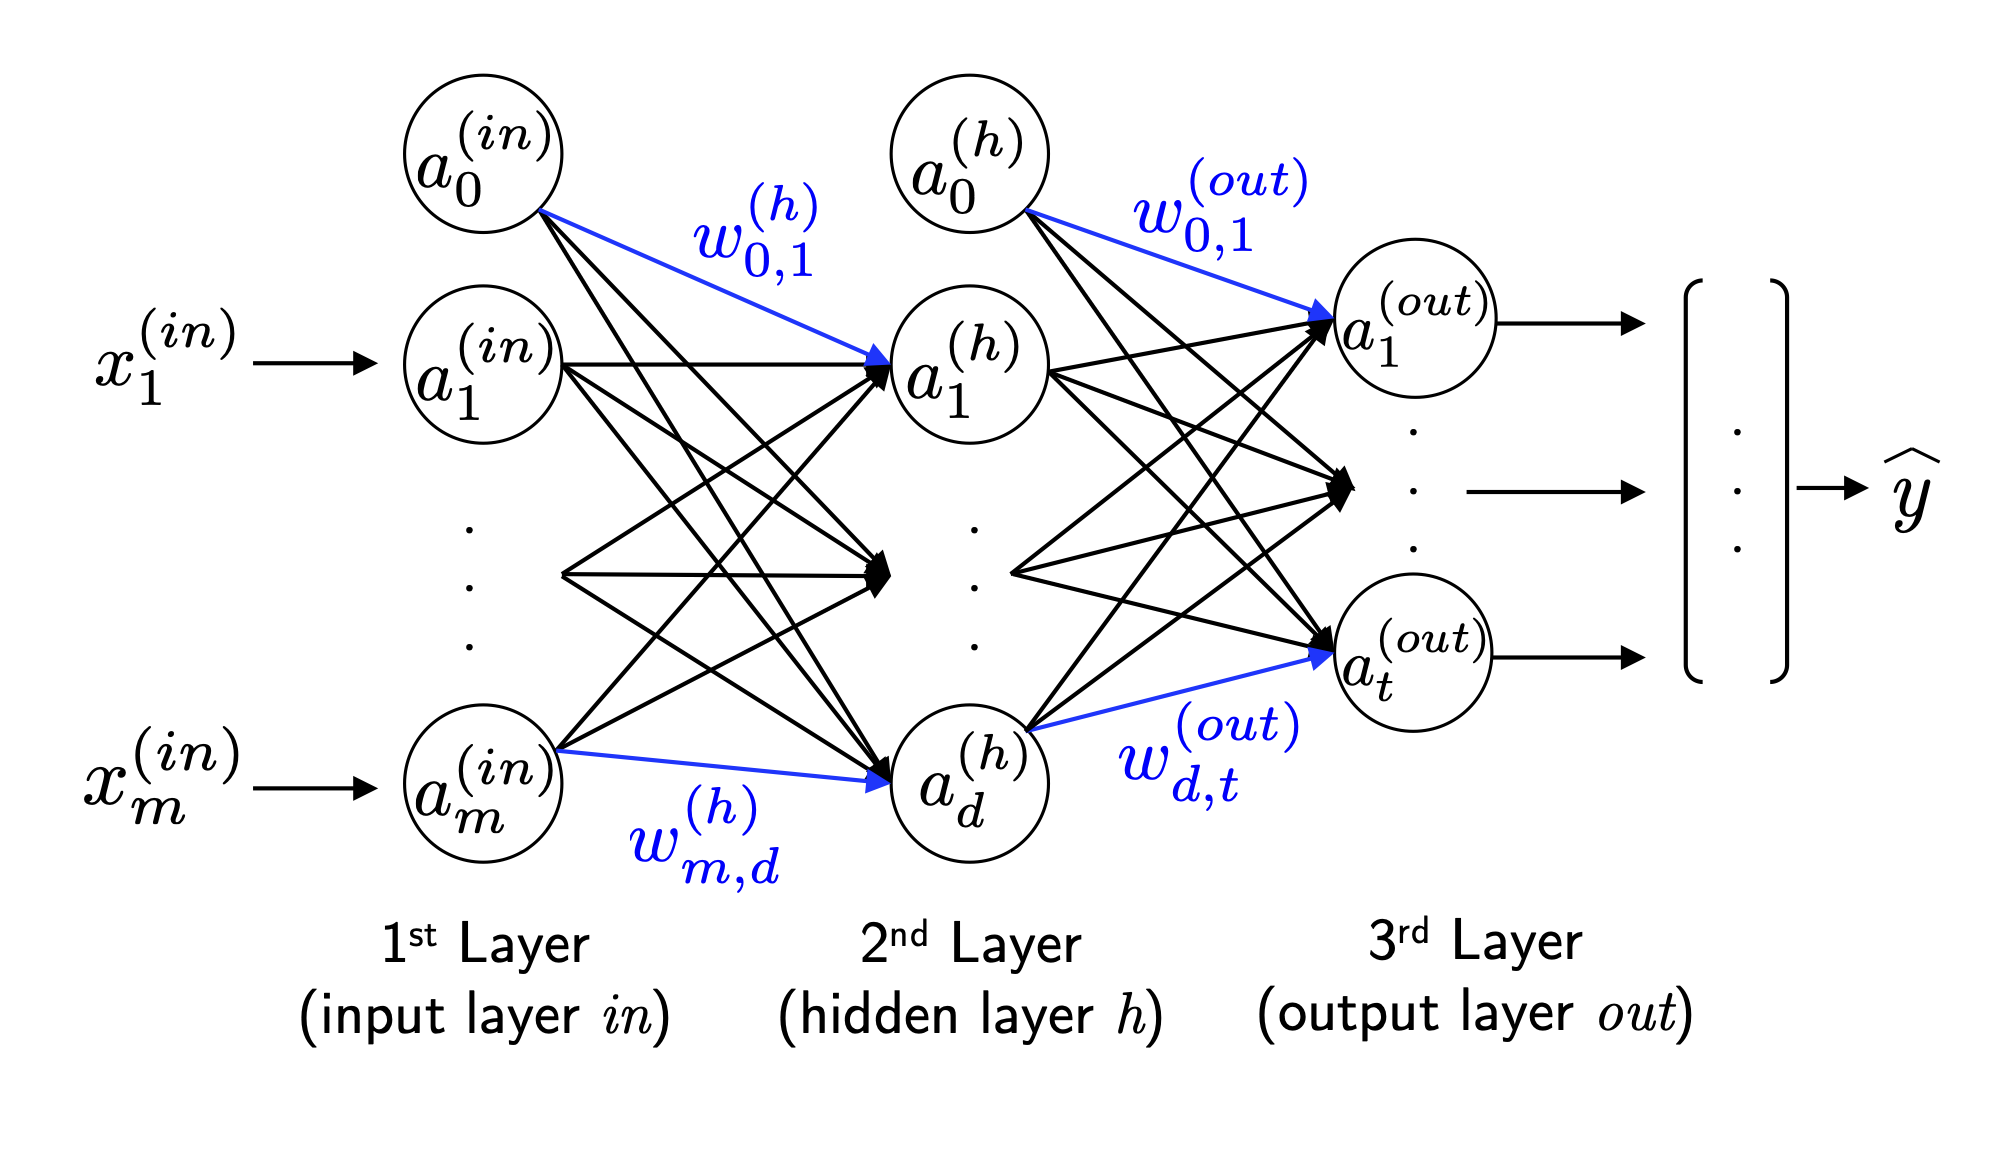
\includegraphics[width = 16cm, height = 9cm]{mlp.png}
\end{center}

Here again, we will consider \underline{ONE} training example.
However, the network has ``t'' activation units in its output
layer. So, the loss function becomes like this:

\[J(w) = -\sum\nolimits_{i = 1}^{1}\sum\nolimits_{j=1}^{t} y_j^{[i]} ln(a_j^{[i]}) + (1 - y_j^{[i]})ln(1 - a_j^{[i]})\]

\vspace{5mm} %5mm vertical space

Here is what the journey of SINGLE of a training example from 
the input layer to the output layer looks like this:

\pagebreak
\[[a_1^{(in)}, a_2^{(in)}, \cdots, a_m^{(in)}]\]
\[\downarrow\]
\[W^{(h)}\]
\[\downarrow\]                  
\[[z_1^{(h)}, z_2^{(h)}, \cdots, z_d^{(h)}]\]
\[\downarrow\]
\[\phi(\bullet)\]
\[\downarrow\]
\[[a_1^{(h)}, a_2^{(h)}, \cdots, a_d^{(h)}]\]
\[\downarrow\]
\[W^{(out)}\]
\[\downarrow\]                  
\[[z_1^{(out)}, z_2^{(out)}, \cdots, z_t^{(out)}]\]
\[\downarrow\]
\[\phi(\bullet)\]
\[\downarrow\]
\[[a_1^{(out)}, a_2^{(out)}, \cdots, a_t^{(out)}]\]
\[\downarrow\]
\[[y_1, y_2, \cdots, y_t]\]
\pagebreak

Notice, the biases have been ignored in the preceding figure.

\vspace{5mm} %5mm vertical space

Let's now draw a tree diagram once again to see how
the variables in $J(W)$ in are related to the weights in
$W^{(out)}$. As you probaby think already, it's pretty similar
to what we had for the 2-2-2 MLP.

\vspace{5mm} %5mm vertical space

\begin{figure}[h!]
    \centering
    \begin{forest}
        for tree={
            l sep=30pt,
            parent anchor=south,
            align=center
        }
            [$J(W)$
                [$y_1^{[i]}$]
                [$a_1^{[i]}$
                    [$z_1^{[i]}$
                        [$w_{1,1}^{(out)}$]
                        [$w_{2,1}^{(out)}$]
                    ]
                ]
                [$y_2^{[i]}$]
                [$a_2^{[i]}$
                    [$z_2^{[i]}$
                        [$w_{1,2}^{(out)}$]
                        [$w_{2,2}^{(out)}$]
                    ]
                ]
            ]
    \end{forest}
\end{figure}

\section{Challenge}

Can you repeat everything we did, but considering $n$ training
examples?
\end{document}